\documentclass[12pt]{article}
\oddsidemargin -0.5in
\evensidemargin -0.5in
\textwidth 7.2in
\topmargin -0.5in
\textheight 8in
\flushbottom

\usepackage[authoryear,round]{natbib} %a package for formatting citations
\usepackage{amsmath} %a package for good looking equations and symbols
\usepackage{algorithm2e} %a package for typesetting algorithms
% \usepackage{caption} %a package for more complex captions for figures/tables/images
\usepackage{subcaption} %extension of the caption package
\usepackage{url} %embedded, clickable links
\usepackage{fullpage} %including this package changes the default margins to use more of the page
\usepackage{graphicx} %package for inline images
\usepackage[usenames]{xcolor} %for adding color text
\usepackage{enumitem} %for nested numbered lists (like in the questions section)
% \usepackage{hyperref}
% \usepackage{amsfonts}

\newcommand{\nextproblem}{
	\vfill
	\pagebreak
}
\setlist[itemize]{noitemsep, topsep=1pt}
\graphicspath{{plots/final/}}

\begin{document}

\begin{center}
    \textbf{CS 4641 Machine Learning \\ Bojun Yang | Section B Homework 2 Writeup}
\end{center}

\begin{enumerate}[noitemsep,topsep=1pt]
\item KNN Analysis
\begin{enumerate}[noitemsep,topsep=1pt]
    \item Euclidean Distance
    \begin{enumerate}[noitemsep,topsep=1pt]
        \item HTRU2 | Best individual: 0.02094972067039106,(k=80)
        \\ A good range for k is [6,15]. The testing data loss within this range has reached it's lowest
        and we are not overfitting the training data yet. 
        \\ 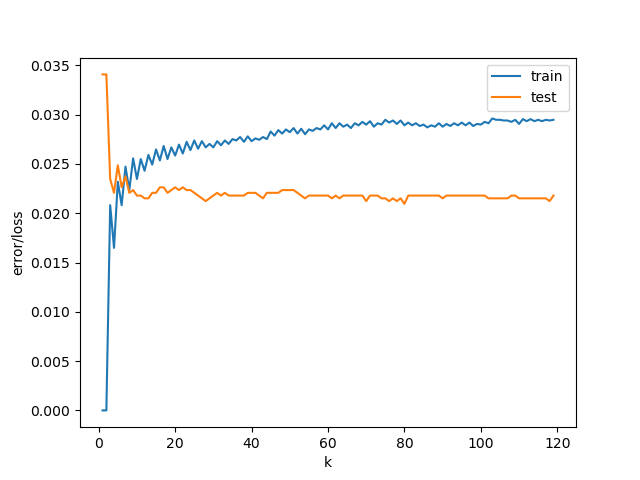
\includegraphics[height=0.4\textheight]{HTRU2_euc}
        \\ 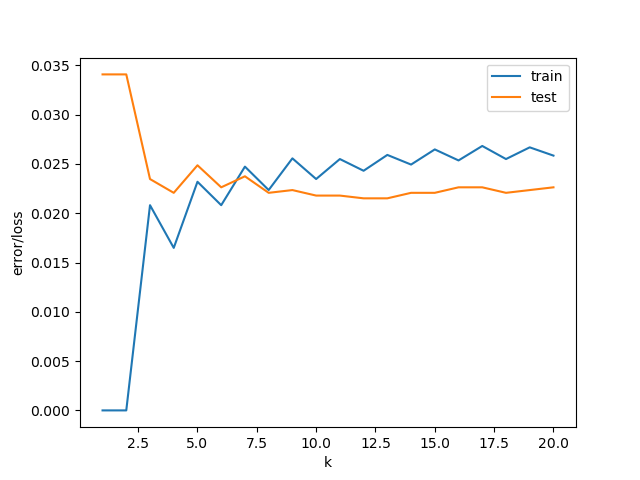
\includegraphics[height=0.4\textheight]{HTRU2_euc20}
        \nextproblem
        \item iris | Best individual: 0.03333333333333333,(k=1)
        \\ A good range for k seems to be around k = 15 or k = 1. There is a significant decrease in loss for the
        testing data set here. It is difficult to choose a k for this dataset since there isn't a clear
        decreasing loss trend for the testing data set. We know that k values above 70 are definitely 
        unideal because the loss increases dramatically and plateaus.
        \\ 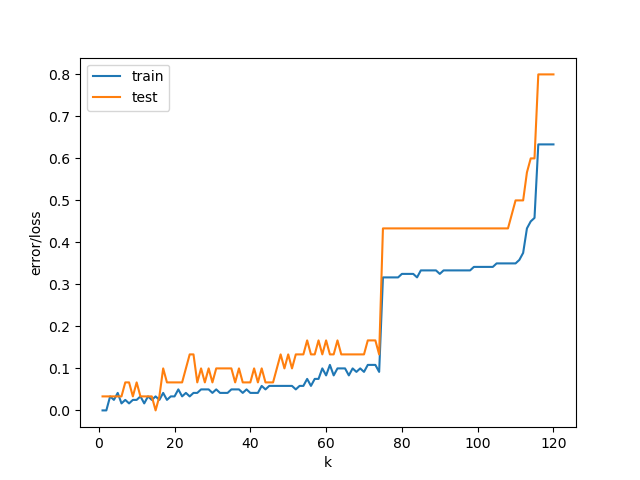
\includegraphics[height=0.5\textheight]{iris_euc}
        \nextproblem
        \item optdigits | Best individual: 0.017807456872565387,(k=4)
        \\ A good range for k is [4,10]. Looking at the first graph, we see that the loss for testing data
        is lowest from k = (0,20]. Zooming into the graph, we can see that the loss for testing data starts
        to increase at k =10.
        \\ 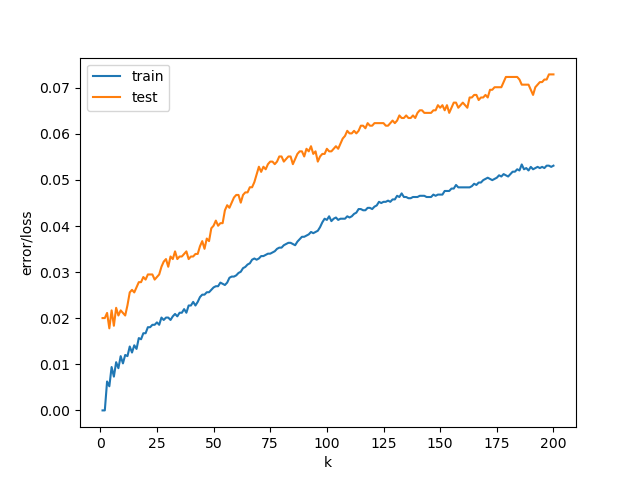
\includegraphics[height=0.4\textheight]{digits_euc}
        \\ 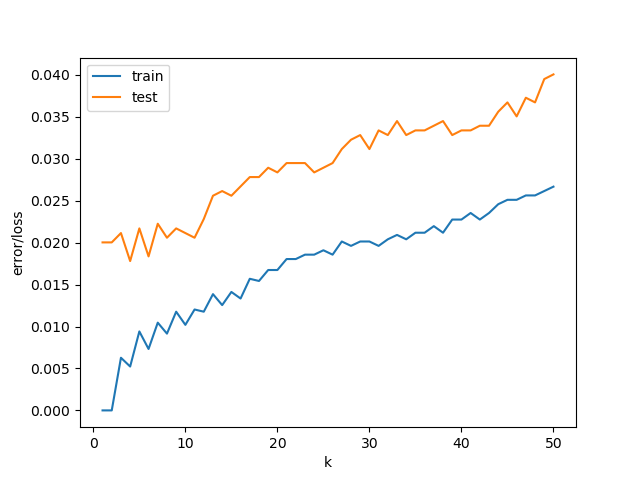
\includegraphics[height=0.4\textheight]{digits_euc50}
    \end{enumerate}
    \nextproblem
    \item Manhattan Distance
    \begin{enumerate}[noitemsep,topsep=1pt]
        \item HTRU2 | Best individual: 0.01983240223463687,(k=26)
        \\ A good range for k is [20, 30]. The testing data loss within this range has reached it's lowest
        and we are not overfitting the training data yet. 
        \\ 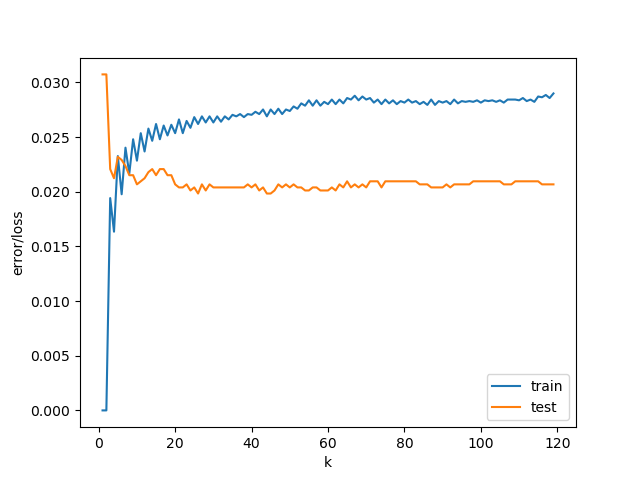
\includegraphics[height=0.4\textheight]{HTRU2_man}
        \\ 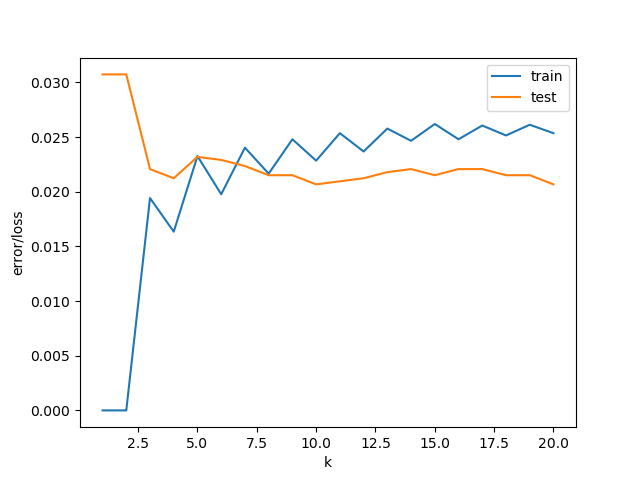
\includegraphics[height=0.4\textheight]{HTRU2_man20}
        \nextproblem
        \item iris | Best individual: 0.03333333333333333,(k=1)
        \\ A good range for k seems to be [1,13]. It is difficult to choose a k for this dataset since there isn't a clear
        decreasing loss trend for the testing data set. We know that k values above 70 are definitely 
        unideal because the loss increases dramatically and plateaus.
        \\ 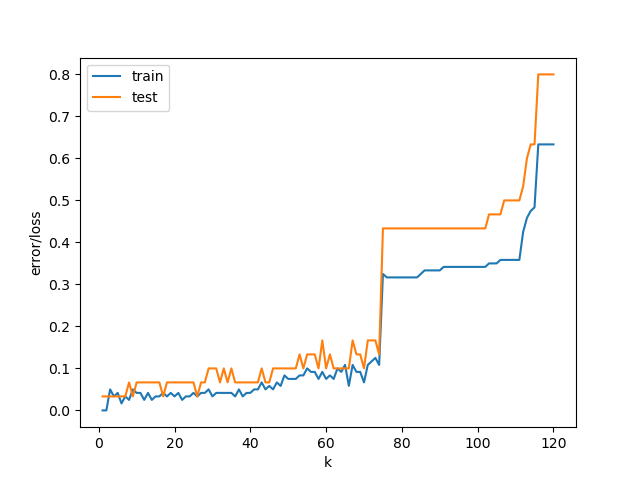
\includegraphics[height=0.5\textheight]{iris_man}
        \nextproblem
        \item optdigits | Best individual: 0.023928770172509738,(k=4)
        \\ A good range for k is [2,8]. Looking at the first graph, we see that the loss for testing data
        is lowest from k = (0,20]. Zooming into the graph, we can see that the loss for testing data starts
        to increase at k =10.
        \\ 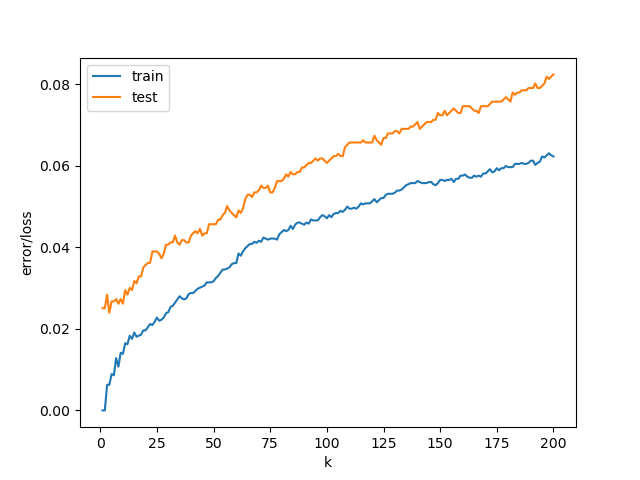
\includegraphics[height=0.4\textheight]{digits_man}
        \\ 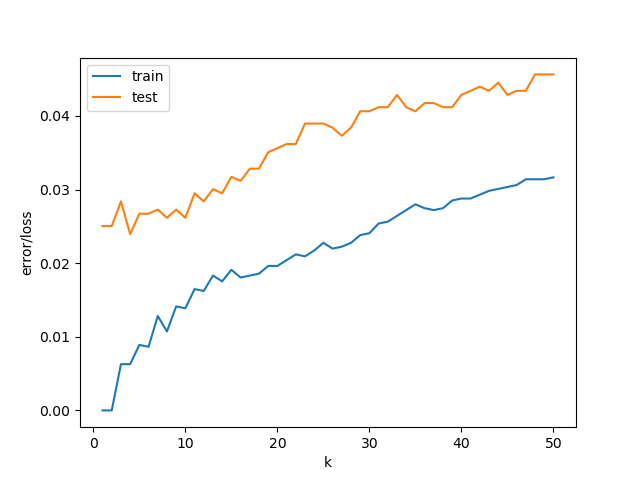
\includegraphics[height=0.4\textheight]{digits_man50}
    \end{enumerate}
    \nextproblem
    \item Mahalanobis Distance
    \begin{enumerate}[noitemsep,topsep=1pt]
        \item HTRU2 | Best individual: 0.01452513966480447,(k=6)
        \\ A good range for k is [4,10]. The testing data loss within this range has reached it's lowest
        and we are not overfitting the training data yet. 
        \\ 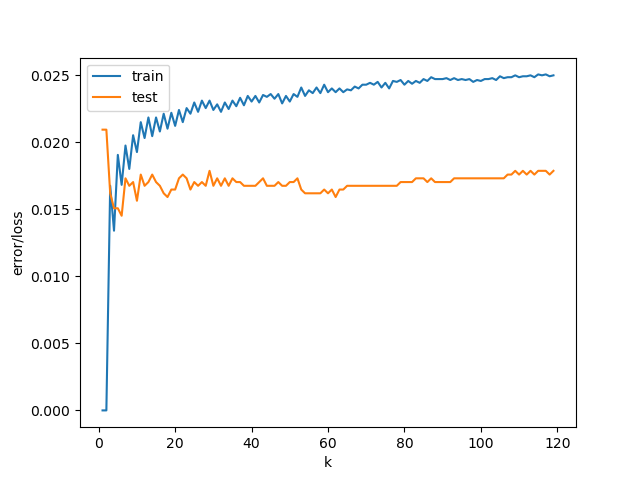
\includegraphics[height=0.4\textheight]{HTRU2_mah}
        \\ 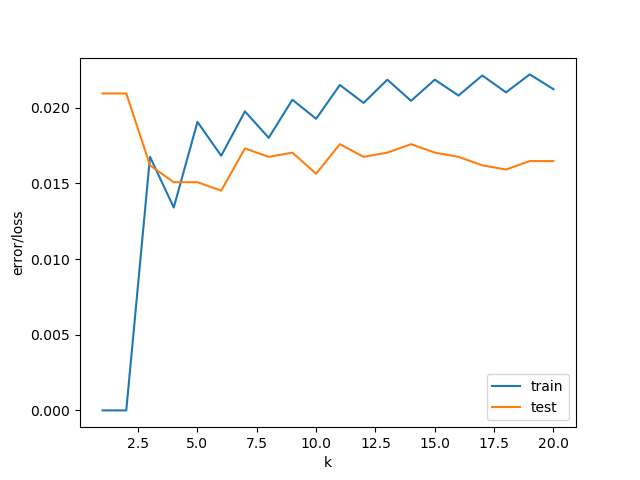
\includegraphics[height=0.4\textheight]{HTRU2_mah20}
        \nextproblem
        \item iris | Best individual: 0.03333333333333333,(k=1)
        \\ A good range for k seems to be [1,15]. It is difficult to choose a k for this dataset since there isn't a clear
        decreasing loss trend for the testing data set. We know that k values above 70 are definitely 
        unideal because the loss increases dramatically and plateaus.
        \\ 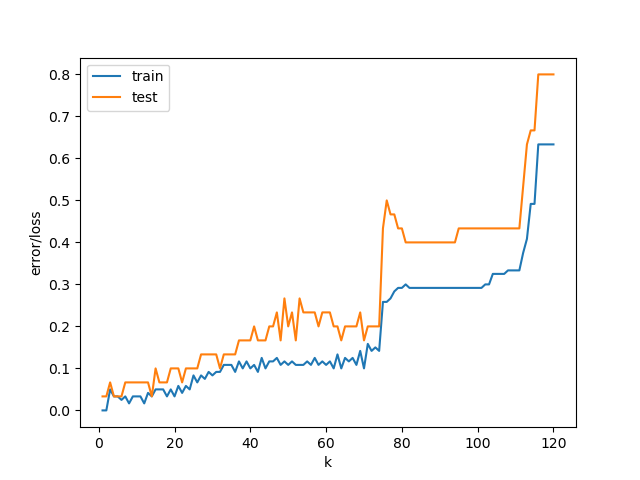
\includegraphics[height=0.5\textheight]{iris_mah}
        \nextproblem
        \item optdigits | Best individual: 0.0333889816360601,(k=3)
        \\ A good range for k is [2,7]. Looking at the first graph, we see that the loss for testing data
        is lowest from k = (0,20]. Zooming into the graph, we can see that the loss for testing data starts
        to increase at k =10.
        \\ 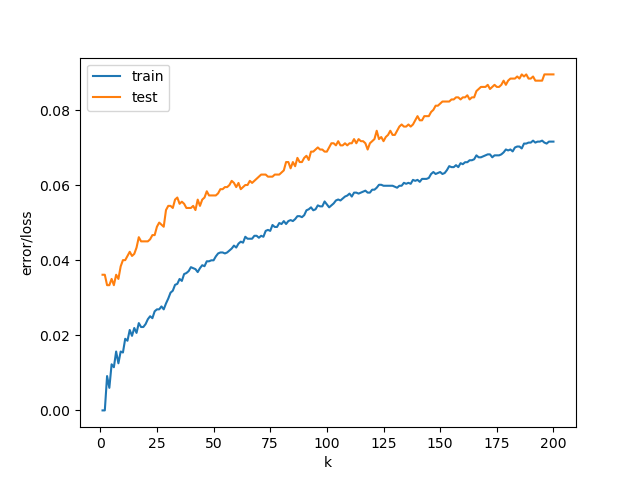
\includegraphics[height=0.4\textheight]{digits_mah}
        \\ 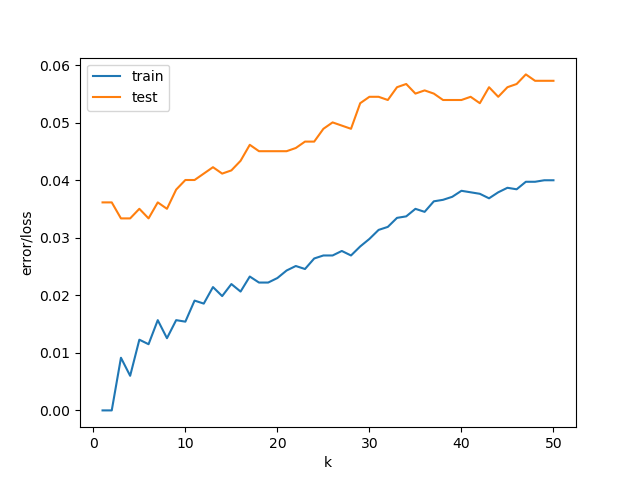
\includegraphics[height=0.4\textheight]{digits_mah50}
    \end{enumerate}
\end{enumerate}
\nextproblem
\item Logistic Regression Analysis
\begin{enumerate}
    \item HTRU2
    \\ Converged, iteration 1109
    \\ HTRU2 LogReg Test score: 0.976536312849162, HTRU2 LogReg Train score: 0.9698281882944545
    \\ Compared to the lowest loss of KNN on HRTU2 (0.0145), Logistic regression falls short with
    about a 0.03 loss. KNN had better performance.
    \item iris
    \\ learner 0: Converged, iteration 14577
    \\ learner 1: Converged, iteration 8816
    \\ learner 2: Converged, iteration 28537
    \\ iris LogReg Test score: 0.9666666666666667, iris LogReg Train score: 0.9666666666666667
    \\ Compared to the lowest loss of KNN on iris (0.03), Logistic regression has a similar performance
    with about a 0.033 loss. However, we should note that the best KNN performances all had k=1, which is
    overfitting.
    \item optdigits
    \\ learner 0: Converged, iteration 2502
    \\ learner 1: Converged, iteration 3376
    \\ learner 2: Converged, iteration 3161
    \\ learner 3: Converged, iteration 3426
    \\ learner 4: Converged, iteration 3790
    \\ learner 5: Converged, iteration 3948
    \\ learner 6: Converged, iteration 2706
    \\ learner 7: Converged, iteration 2894
    \\ learner 8: Converged, iteration 4033
    \\ learner 9: Converged, iteration 4410
    \\ digits LogReg Test score: 0.9365609348914858, digits LogReg Train score: 0.9641642688987706
    \\ Compared to the lowest loss of KNN on optdigits (0.0178), Logistic regression falls short with
    about a 0.07 loss. KNN had better performance.
    \item Analysis
    \\ Logistic regression peroforms well when the data can be linearly separated, a good learning rate is chosen,
    and a good enough initial theta is chosen. 
    HTRU2 is a 8 dimensional dataset with binary class labels. 
    Iris is a 4 dimensional dataset with multi-class labels. 
    Optdigits is a 64 dimensional dataset with multi-class labels.
    logistic regression seems to perform well with HTRU2 and iris. It makes sense for HTRU2 because the line
    is able to use 8 dimensions to fit 2 labels. Similarily with iris (3 unique class labels), logistic regression
    performs well. With optdigits, logistic regression performs the worst possibly due to the increased number
    of labels (10). Based on these reasonings, I don't think that the optdigits dataset is easily linearly separable
    while HTRU2 and iris datasets are. Our learning rate was small enough so that logistic regression converged
    within a reasonable amount of runs and our thetas were initialized to 0, which is good enough. 
\end{enumerate}
\nextproblem
\item Support Vector Machines
\begin{enumerate}
    \item $h_{\mathbf{w},w_0}(\mathbf{x}) = \text{sgn}\left\{ w_0 + \phi(\mathbf{x})^\top \mathbf{w} \right\}$
    \\ $w = \Sigma_{i-=1}^N \alpha^{(i)} y^{(i)}x^{(i)}$
    \\ Kernal trick: $K(x^{(i)},x) = \phi(x^{(i)})\phi(\mathbf{x})^\top$
    \\ Apply feature transform to x: $w = \Sigma_{i=1}^N \alpha^{(i)} y^{(i)} \phi(x^{(i)})$
    \\ $\phi(\mathbf{x})^\top \mathbf{w}$ = $\phi(\mathbf{x})^\top \Sigma_{i=1}^N \alpha^{(i)} y^{(i)} \phi(x^{(i)}) 
    = \Sigma_{i=1}^N \alpha^{(i)} y^{(i)} \phi(x^{(i)})\phi(\mathbf{x})^\top 
    = \Sigma_{i=1}^N \alpha^{(i)} y^{(i)} K(x^{(i)},x)$
    \\ The Kernel computes the inner product of $x^T x'$ with a function k. 
    Using the kernelized version of SVMs as seen above, we don't have to explicitly calculate $\phi(x) \phi(x')^T$.
    This allows us to operate in higher dimensions by using an easy to compute kernel function 
    instead of computing a potentially high-dimensional transform. $\alpha^{(i)}$ determine which points 
    are the support vectors that determine the decision boundary. Support vectors have an $\alpha^{(i)} > 0$,
    which means if a point is not a support vector, it's $\alpha^{(i)} = 0$. This effectively removes
    this point from the calculation of $h_{\mathbf{w},w_0}(\mathbf{x})$. 

    \item
    $k_{lin}(\mathbf{x},\mathbf{x}^\prime): D$ dimensions 
    \\ The vectors in the kernel are the original vectors. The dimensions will stay the same in $\phi$ 
    because a linear transform does not increase the number dimensions. \\
    \\$k_{poly}(\mathbf{x},\mathbf{x}^\prime): {(D+M) \choose M}$ dimensions
    \\ e.g. $(a+b+c+d+1)^2, D=4, M=2$
    \\ squaring a polynomial with 4 variables results in a new polynomial with ${6 \choose 2}$ terms.
    Generalizing to the binomial theorem: a polynomial with D terms raised to the M'th power results in a new polynomial with ${(M+D) \choose M}$ terms. \\
    \\$k_{exp}(\mathbf{x},\mathbf{x}^\prime)$: infinite dimensions
    \\ The taylor series expansion of $e^z = 1 + \frac{1}{1!}z + \frac{1}{2!}z^2 + \frac{1}{3!}z^3 + ... + \frac{1}{\infty !}z^{\infty}$
    \\ Seeing how the power of z goes to infinity, this kernel is similar to a polynomial kernel with D = $\infty$.
    Therefore, the number of dimensions this feature transform calculates is infinity. 

    \item Find vector $v$ parallel to $\mathbf{w}$ \\
    \\ $x_1=0, x_2=\sqrt{2}, y_1=-1, y_2=1$ 
    \\ $\phi(x)=[1,\sqrt{2}x,x^2]$ 
    \\ $\phi(x_1)=[1,0,0], \phi(x_2)=[0,2,2], v=\phi(x_2) - \phi(x_1) = [0,2,2]$
    \item find r, value of the margin achieved by $\mathbf{w}$
    \\ $r = \sqrt{0^2+2^2+2^2} = \sqrt{8} $
    \item find $\mathbf{w}$
    \\ $||\mathbf{w}|| = \frac{2}{r} = \frac{2}{\sqrt{8}}$ 
    \\ $\mathbf{w} = \frac{||\mathbf{w}||}{r}v = \frac{\frac{2}{\sqrt{8}}}{\sqrt{8}}v = 
    \frac{1}{4} <0,2,2> = <0, \frac{1}{2}, \frac{1}{2}> $
    \item find $w_0$
    \\ I don't writeout $\mathbf{w}^T$ and $\phi(x)$ because they are defined in my part c and e.
    \\ $-1(\mathbf{w}^T \phi(x_1) + w_0) = -1(0 + w_0) = -w_0 \geq 1 \rightarrow w_0 \leq -1$ 
    \\ $1(\mathbf{w}^T\phi(x_2) + w_0) = 1(2 + w_0) = 2 + w_0 \geq 1 \rightarrow w_0 \geq -1$
    \\ Therefore $w_0 = -1$
    \item Write down discriminant function 
    \\ $f(x) = w_0 + \mathbf{w}^T\phi(x)  = -1 + \frac{\sqrt{2}}{2}x + \frac{x^2}{2}$

\end{enumerate}
\end{enumerate}

\end{document}

